\documentclass[12pt,letterpaper]{article}

\usepackage{ucs}
\usepackage[utf8x]{inputenc}
\usepackage[T1]{fontenc}
\usepackage{amsmath}
\usepackage{amsfonts}
\usepackage{amssymb}
\usepackage{graphicx}
\usepackage{fullpage}

\usepackage[colorlinks=true, 
            pdfstartview=FitV, 
            linkcolor=black, 
            citecolor=black,
            urlcolor=black]{hyperref}

\date{\today}
\author{Charles Varin}
\title{Optical response of a dipolar medium for integration with the finite-differences time-domain method for solving the Maxwell equations}

\begin{document}
\maketitle 
\tableofcontents
\section{Introduction}\label{intro}
In the presence of a medium with an electric susceptibility (but no free charges), the evolution of the electric and magnetic field vectors $\mathbf{E}$ and $\mathbf{H}$ is given by the following Maxwell equation:
\begin{subequations}\label{eq:maxwell}
  \begin{align}\label{eq:maxwell1}
   \frac{\partial\mathbf{E}}{\partial t} &=\frac{1}{\epsilon}\nabla\times\mathbf{H}-\frac{1}{\epsilon}\frac{\partial\mathbf{P}}{\partial t},\\
   \frac{\partial\mathbf{H}}{\partial t} &=-\frac{1}{\mu_0}\nabla\times\mathbf{E},\label{eq:maxwell2}
  \end{align}
\end{subequations}
where $c = 1/\sqrt{\epsilon\mu_0}$ with $\epsilon = \epsilon_0\epsilon_r$. In the next sections, a model for the temporal evolution of the polarization $\mathbf{P}$ of a dipolar medium is presented. For general details regarding to the finite-differences time-domain (FDTD) method for solving Eqs. \eqref{eq:maxwell}, see \cite{sullivan2000,taflove2005}.

\section{Static response of a dipolar medium}\label{static}
A dipolar medium is composed of molecules that possess a permanent dipole moment and whose polarizability is anisotropic. In a static electric field, initially disordered molecules will tend to align along the field lines leading to an average polarization. Models for the static response associated with the permanent dipole moment and the anisotropic susceptibility can be found in \cite{jackson1999,hook1991} and \cite{boyd2008}, respectively. We here put those two models together and see that the result is not the same as if they were treated as independent contributions. 

A molecule in a static electric field rotates to align along the electric field lines. The potential energy of the molecule in the field is  \cite{boyd2008,bonin1997}:
\begin{align}\label{eq:potential}
U &=-\mathbf{p}_0\cdot\mathbf{E} - \frac{1}{2}\mathbf{E}\cdot\mathbf{\boldsymbol\alpha}\cdot\mathbf{E}\nonumber\\
&= -p_0E\cos\theta-\frac{1}{2}\left[\alpha_\bot + (\alpha_\parallel - \alpha_\bot)\cos^2\theta\right]E^2,
\end{align}
where $p_0$ is the permanent dipole moment, $\alpha = \alpha_\bot + (\alpha_\parallel - \alpha_\bot)\cos^2\theta$ the molecular polarizability (see Eq. (4.4.8) of \cite{boyd2008}), and $\theta$ the angle between the molecular axis and $E$. The corresponding molecular polarization is thus:
\begin{equation}\label{eq:single_pol}
 p = p_0\cos\theta+\left[\alpha_\bot + (\alpha_\parallel - \alpha_\bot)\cos^2\theta\right]E,
\end{equation}
In the equations above, $\alpha_\bot$ and $\alpha_\parallel$ are, respectively, the first-order molecular polarizabilities perpendicular and parallel to the molecular axis,i.e., perpendicular and parallel to the vector $\mathbf{p}_0$.

For a collection of molecules, the total polarization is the average over all the molecules times the number of molecules per unit volume:
\begin{equation}\label{eq:total_pol}
 P=N<p>=N\left\lbrace p_0<\cos\theta>+\left[\alpha_\bot + (\alpha_\parallel - \alpha_\bot)<\cos^2\theta>\right]E\right\rbrace.
\end{equation}
At equilibrium and in the limit where the molecules are not interacting too strongly, the molecular orientations are given by a Boltzmann distribution and
\begin{subequations}\label{eq:statistics}
 \begin{align}
  <\cos\theta>&=\frac{\int_0^\pi\cos\theta\exp(-U/k_BT)\sin\theta d\theta}{\int_0^\pi\exp(-U/k_BT)\sin\theta d\theta},\\
  <\cos^2\theta>&=\frac{\int_0^\pi\cos^2\theta\exp(-U/k_BT)\sin\theta d\theta}{\int_0^\pi\exp(-U/k_BT)\sin\theta d\theta},
 \end{align}
\end{subequations}
where $U$ is a function of $\theta$ [see Eq. \eqref{eq:potential}]. 

Analytical solutions of Eqs.~\eqref{eq:total_pol} and \eqref{eq:statistics} for the case where the polarizability is zero ($\alpha_\bot = \alpha_\parallel=0$) can be found in \cite{hook1991} (Sec. 9.1.3) and \cite{jackson1999} (Sec. 4.6). The solution for $p_0 = 0$ can be found in \cite{boyd2008} (Sec. 4.4). General solutions ($p_0\neq 0$, $\alpha_\bot\neq 0$, and $\alpha_\parallel\neq 0$) were found numerically and are compared with the analytical formulas in Fig. \ref{fig:stat_pol}. It is thus observed that the material response is in general nonlinear, excepted for small field amplitudes ($E\rightarrow 0$).

\begin{figure}[ht]
    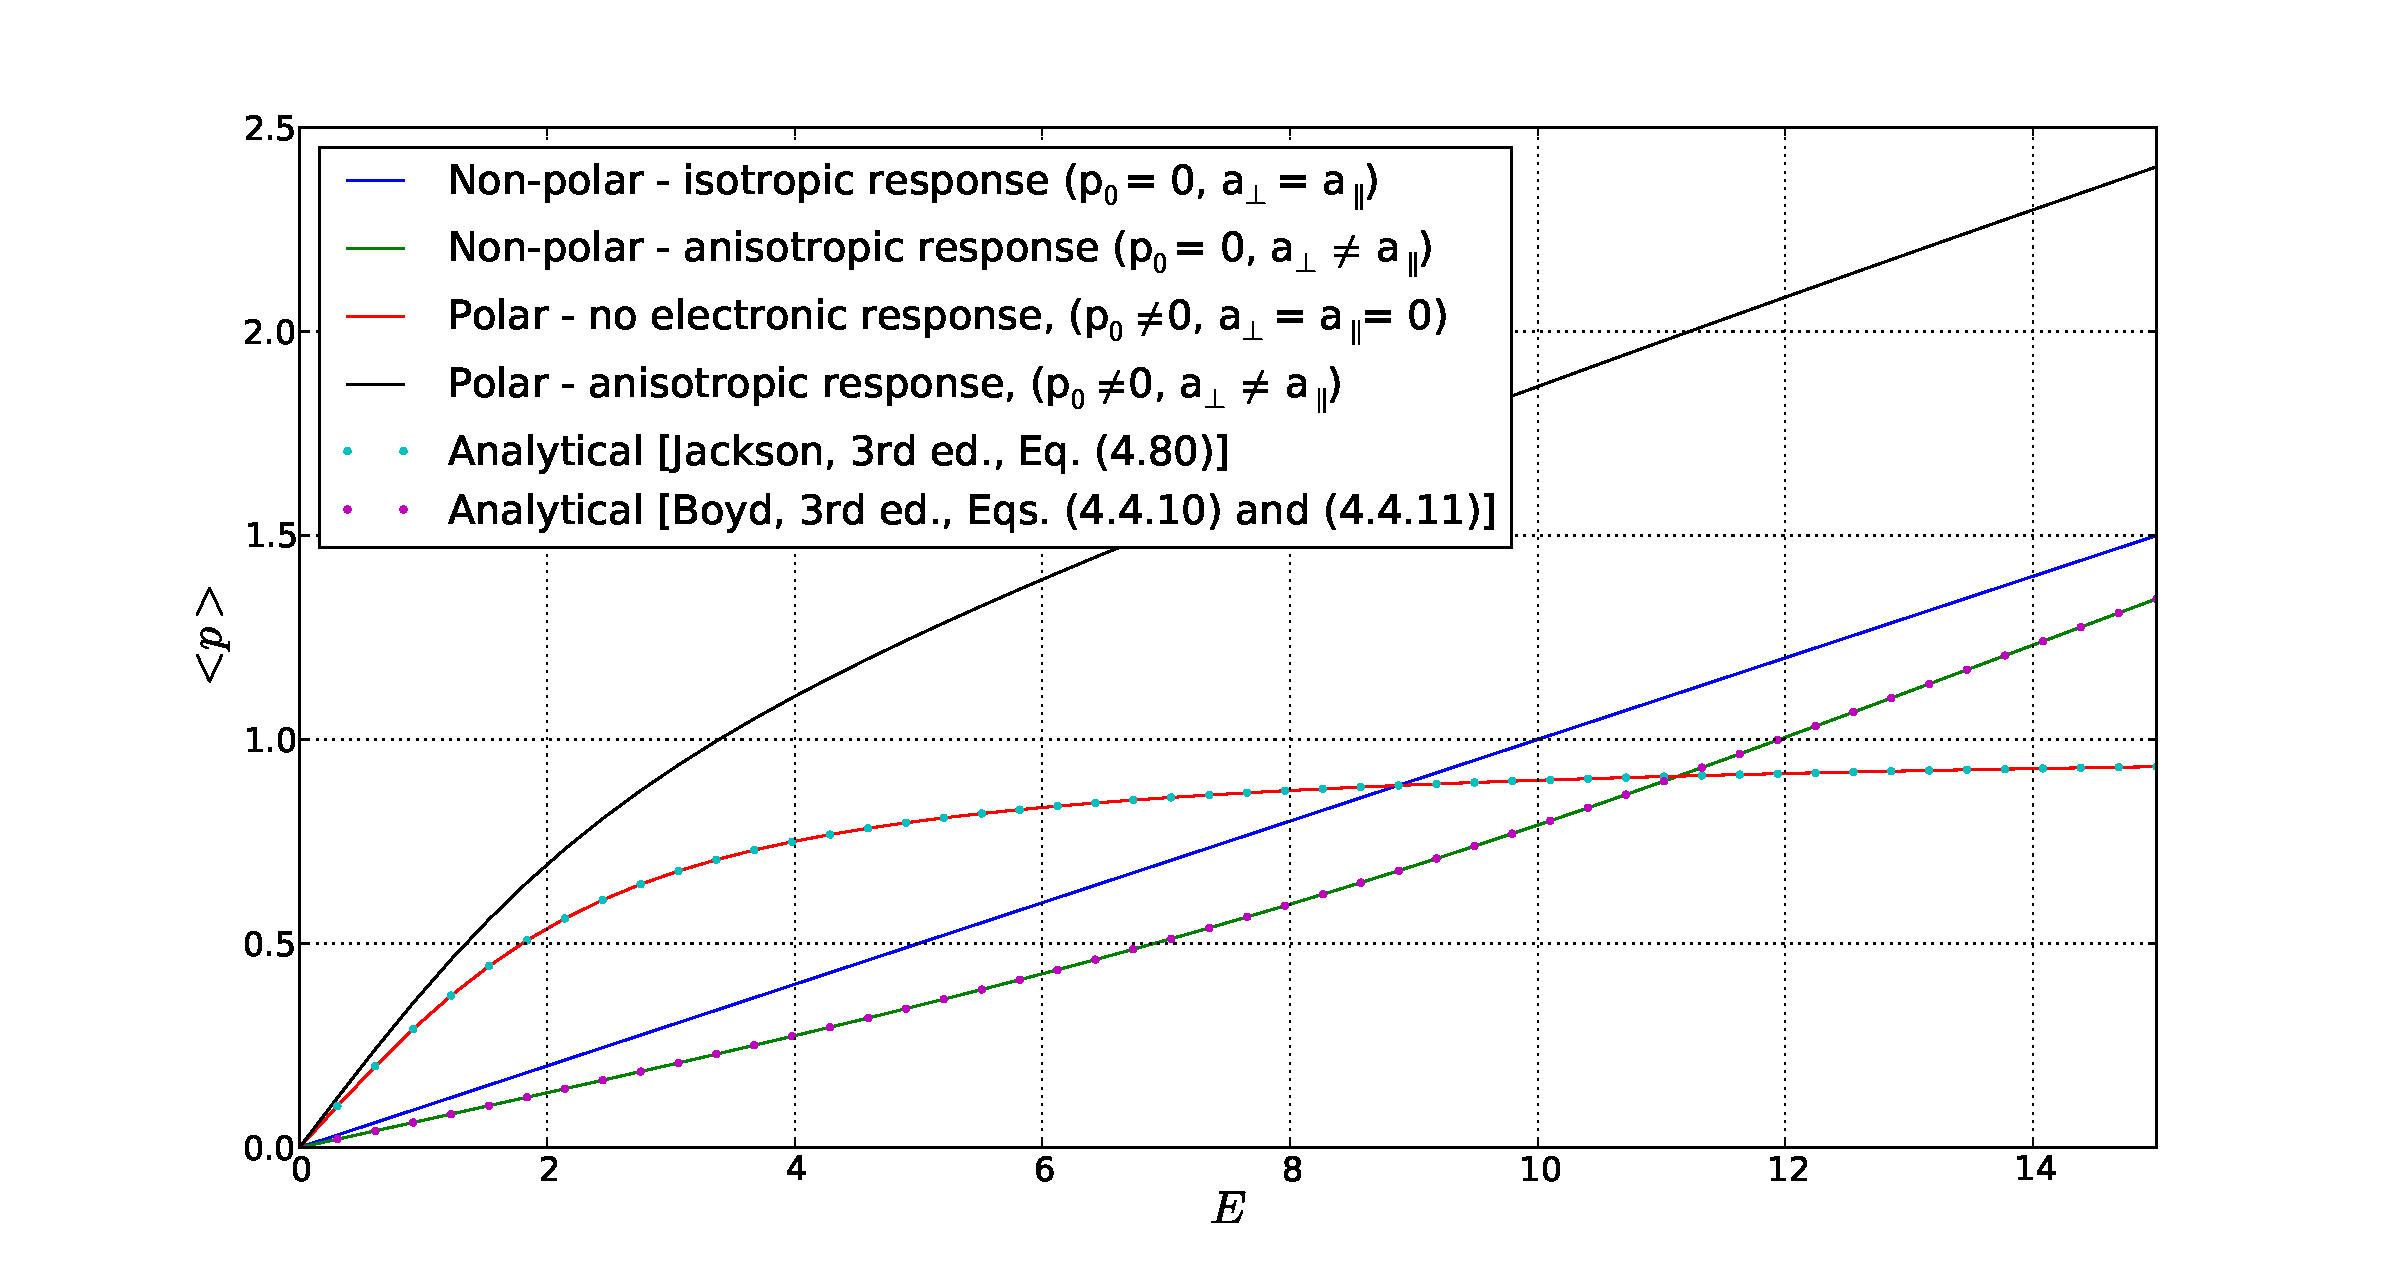
\includegraphics[width=17.2cm]{static_polarization.pdf}
    \caption{Average molecular polarization at equilibrium as a function of the electric field. For a polar material ($p_0\neq 0$), the response is nonlinear. Saturation occurs when the field is strong enough to align the molecules completely.}
    \label{fig:stat_pol}
\end{figure} 

For three-dimensional problems, the potential can be written as 
\begin{align}\label{eq:potential_altern}
U &= \sum_{i=x,y,z} p_0E_i\cos\theta_i+\frac{1}{2}\left[\alpha_\bot + (\alpha_\parallel - \alpha_\bot)\cos^2\theta_i\right]E_i^2,
\end{align}
where $\theta_i$ are the direction angles with respect to the $x,y,$ and $z$ axes. Each $<\cos\theta_i>$ and $<\cos^2\theta_i>$ can be calculated independently using Eqs. \eqref{eq:statistics}. The components of the material polarization are then:
\begin{equation}\label{eq:pol_components}
 P_i=N<p_i>=N\left\lbrace p_0<\cos\theta_i>+\frac{1}{2}\left[\alpha_\bot + (\alpha_\parallel - \alpha_\bot)<\cos^2\theta_i>\right]E_i\right\rbrace.
\end{equation}

\section{Weak-field (linear) response}\label{weak_field}
Before going any further, we define the material response in the limit where the field is weak, i.e., when $E\rightarrow 0$. In other words, we will find the linear response so that $<p>_0=<\alpha>_0 E$. For that, we expand the exponential function of the Boltzmann distribution to the first order in $E$:
\begin{align}\label{eq:exponential_first_order}
  \exp(-U/k_BT)\simeq 1-\frac{U}{k_BT} = 1+\frac{p_0E}{k_BT}\cos\theta + O(E^2).
\end{align}
Using this expression in Eqs. \eqref{eq:statistics} then gives:
\begin{subequations}\label{eq:statistics_weak_field}
 \begin{align}
  <\cos\theta>&=\frac{p_0 E}{3k_BT},\\
  <\cos^2\theta>&=\frac{1}{3},
 \end{align}
\end{subequations}
and we find
\begin{equation}\label{eq:total_pol_weak_field}
 <p>_0=\left[\frac{p_0^2 }{3k_BT}+\left(\frac{1}{3}\alpha_\parallel + \frac{2}{3}\alpha_\bot\right)\right] E,
\end{equation}
in agreement with \cite{jackson1999,hook1991,boyd2008,bonin1997}. This can be converted into a linear refractive index ($n_0$), or linear relative electric permittivity ($\epsilon_r$) \cite{boyd2008}.

\section{Nonlinear response}\label{non_linear}
As seen in Fig. \ref{fig:stat_pol}, the response of a dipolar material is nonlinear. A general molecular polarization can thus be written $<p>=<\alpha>_0E + <p>_{NL}$, where $NL$ stands for \textit{nonlinear}. The mathematical form of $<p>_{NL}$ is not necessarily a simple analytical expression. But it is easily obtained by calculating the full polarization numerically and subtracting the linear response, i.e., 
\begin{align}\label{eq:non_linear_pol}
 <p>_{NL} &= <p> - <p>_0,
\end{align}
Then, the electric displacement is written:
\begin{align}\label{eq:electric_displacement}
 D &= \epsilon_r\epsilon_0 E + N<p>_{NL}.
\end{align}
The form of Eq. \eqref{eq:electric_displacement} is desired to perform stable numerical solutions of the Maxwell equations with the FDTD method \cite{sullivan2000,taflove2005}.

As an example, we expanded Eq. \eqref{eq:exponential_first_order} up to second order in $E$ and  
\begin{align}\label{eq:exponential_second_order}
  \exp(-U/k_BT)\simeq 1+\frac{p_0E}{k_BT}\cos\theta+ \frac{p_0^2E^2}{2\,k_B^2T^2}\cos^2\theta + \frac{\alpha_\bot E^2}{2k_BT} +
\frac{\left(\alpha_\parallel - \alpha_\bot\right) E^2}{2k_BT}\cos^2\theta+ O(E^3),
\end{align}
Then, when integrating term by term, is obtained:

% From a calculation similar than that of Sec. \ref{weak_field}, we obtained:
\begin{subequations}\label{eq:statistics_second_order_cos}
 \begin{align}
  <\cos\theta>&=\frac{p_0E/(3k_BT)}{1+\left(\alpha_\parallel/3+2\alpha_\bot/3\right){E}^{2}/k_BT+{p_0}^{2}{E}^{2}/6(k_BT)^{2}},\\
  &\simeq \frac{p_0E}{3k_BT}\left[1-\left(\frac{1}{3}\alpha_\parallel+\frac{2}{3}\alpha_\bot\right)\frac{E^{2}}{k_BT}-\frac{{p_0}^{2}{E}^{2}}{6(k_BT)^{2}}\right],\\
  &\simeq \frac{p_0E}{3k_BT} + O(E^3),	
 \end{align}
\end{subequations}
\begin{subequations}\label{eq:statistics_second_order_cos_sqr}
 \begin{align}
  <\cos^2\theta>&=\frac{1/3 + \left(6\alpha_\parallel +4\alpha_\bot\right)E^2/30k_BT+p_0^2E^2/10(k_BT)^{2}}{1+\left(\alpha_\parallel/3+2\alpha_\bot/3\right){E}^{2}/k_BT+{p_0}^{2}{E}^{2}/6(k_BT)^{2}},\\
&\simeq \frac{1}{3} - \left[\left(\frac{1}{3}\alpha_\parallel+\frac{2}{3}\alpha_\bot\right)\frac{1}{3k_BT}+\frac{{p_0}^{2}}{18(k_BT)^{2}}\right]E^2 + O(E^4),
 \end{align}
\end{subequations}
and
\begin{align}\label{eq:total_pol_second_order}
 <p>&\simeq\left[\frac{p_0^2}{3k_BT}+\left(\frac{1}{3}\alpha_\parallel+\frac{2}{3}\alpha_\bot\right)\right]E - (\alpha_\parallel - \alpha_\bot)\left[\left(\frac{1}{3}\alpha_\parallel+\frac{2}{3}\alpha_\bot\right)\frac{1}{3k_BT}+\frac{{p_0}^{2}}{18(k_BT)^{2}}\right]E^3\nonumber\\ 
 &\qquad + ...
\end{align}
The equation has the form $<p>=<\alpha>_0E + <\alpha>_{NL}E$, where $<\alpha>_{NL}$ depends on $E^2$, i.e., on the laser intensity. The intensity dependent polarizability is responsible for the optical Kerr effect and other nonlinear optical phenomena \cite{boyd2008}.

% the molecular polarizability up to the second order in $E$: $<p>=<\alpha>_0E + <\alpha>_1E^2$

\section{Time evolution of the molecular polarizability}\label{time}

\bibliographystyle{unsrt} 
\bibliography{dipmed}
\end{document}
